% Options for packages loaded elsewhere
\PassOptionsToPackage{unicode}{hyperref}
\PassOptionsToPackage{hyphens}{url}
%
\documentclass[
  a4paper,
  11pt,
  twocolumn]{article}
\usepackage{amsmath,amssymb}
\usepackage{iftex}
\ifPDFTeX
  \usepackage[T1]{fontenc}
  \usepackage[utf8]{inputenc}
  \usepackage{textcomp} % provide euro and other symbols
\else % if luatex or xetex
  \usepackage{unicode-math} % this also loads fontspec
  \defaultfontfeatures{Scale=MatchLowercase}
  \defaultfontfeatures[\rmfamily]{Ligatures=TeX,Scale=1}
\fi
\usepackage{lmodern}
\ifPDFTeX\else
  % xetex/luatex font selection
\fi
% Use upquote if available, for straight quotes in verbatim environments
\IfFileExists{upquote.sty}{\usepackage{upquote}}{}
\IfFileExists{microtype.sty}{% use microtype if available
  \usepackage[]{microtype}
  \UseMicrotypeSet[protrusion]{basicmath} % disable protrusion for tt fonts
}{}
\makeatletter
\@ifundefined{KOMAClassName}{% if non-KOMA class
  \IfFileExists{parskip.sty}{%
    \usepackage{parskip}
  }{% else
    \setlength{\parindent}{0pt}
    \setlength{\parskip}{6pt plus 2pt minus 1pt}}
}{% if KOMA class
  \KOMAoptions{parskip=half}}
\makeatother
\usepackage{xcolor}
\usepackage{graphicx}
\makeatletter
\def\maxwidth{\ifdim\Gin@nat@width>\linewidth\linewidth\else\Gin@nat@width\fi}
\def\maxheight{\ifdim\Gin@nat@height>\textheight\textheight\else\Gin@nat@height\fi}
\makeatother
% Scale images if necessary, so that they will not overflow the page
% margins by default, and it is still possible to overwrite the defaults
% using explicit options in \includegraphics[width, height, ...]{}
\setkeys{Gin}{width=\maxwidth,height=\maxheight,keepaspectratio}
% Set default figure placement to htbp
\makeatletter
\def\fps@figure{htbp}
\makeatother
\setlength{\emergencystretch}{3em} % prevent overfull lines
\providecommand{\tightlist}{%
  \setlength{\itemsep}{0pt}\setlength{\parskip}{0pt}}
\setcounter{secnumdepth}{5}
%------------------------------------------------------------------------------%
% PAPER TEMPLATE FOR ICPHS 2023 Prague                                         %
%                                                                              %
% Original template downloaded from:                                           %
% http://www.icphs2023.org/call-for-papers/                                    %
%                                                                              %
% Reformatted to work with Rmarkdown and R by:                                 %
% Joseph V. Casillas | Rutgers Univesity |11/11/2022                           %
%                                                                              %
% Available for download at:                                                   %
% https://github.com/jvcasillas/icphs2023_rmd_template                         %
%------------------------------------------------------------------------------%



% Packages
\usepackage{./includes/tex/icphs2023}
\usepackage{metalogo} 
\usepackage{epstopdf}
\usepackage{tipa}

% Links and urls must be black
%\hypersetup{urlcolor=black, citecolor=black, linkcolor=black}


% Packages removed from icphs2023.sty because of conflicts
% They have been added to the .Rmd yaml front matter
% \usepackage[latin1]{inputenc}
% \usepackage[T1]{fontenc}
% \usepackage[leqno,fleqn]{amsmath}
\usepackage[utf8]{inputenc}
\usepackage[T1]{fontenc}
\ifLuaTeX
  \usepackage{selnolig}  % disable illegal ligatures
\fi
\IfFileExists{bookmark.sty}{\usepackage{bookmark}}{\usepackage{hyperref}}
\IfFileExists{xurl.sty}{\usepackage{xurl}}{} % add URL line breaks if available
\urlstyle{same}
\hypersetup{
  hidelinks,
  pdfcreator={LaTeX via pandoc}}

\author{}
\date{\vspace{-2.5em}}

\begin{document}

\title{Lateralization of the simple vibrant /r/ to /l/ in Puerto Rican diaspora}
\author{Yhosep Barba}
\organization{Rutgers University}
\email{y.barba@rutgers.edu}


\maketitle

\begin{abstract}
This paper analyzes the production of the lateralization of the simple vibrant /r/ to /l/  within four Puerto Rican women residing in North Carolina. Throughout a reading out-loud task, F3 and F4 trajectories are examined to determine the nature of lambdacism.
\end{abstract}

\keywords{lambdacism, lateralization, accommodation, formants, tap}


\section{Introduction}

This article delves into sociocultural dynamics and linguistic
experiences of four Puerto Rican women living in North Carolina. Here, I
present insights into the intersection of identity, indexicality,
language, and social context. Through the examination of open-ended
interviews and the acoustic analysis of the lateralization of the simple
vibrant /r/ to /l/ in final syllable and word of four participants, this
article aims to show the complexities of language use, negotiation of
identity, and responses to social dynamics in a multicultural setting.
Thus, the acoustic analysis offers a window into phonetic variation
within the Puerto Rican diaspora, showing differences in articulation
strategies and formant trajectories.

\section{Literature Review}

\subsection{Spanish in Puerto Rico}

The Hispanic Antilles, an archipelago that extends from the eastern tip
of Yucatan Peninsula and the southern segment of Florida to the coast of
Venezuela, comprises the Greater and Lesser Antilles. These include
Spanish-speaking countries such as Cuba, the Dominican Republic, and
Puerto Rico (Alba, 2016). Despite being geographically dispersed across
different islands and, additionally, including diverse cultures, there
is a shared perception that they all have the same dialect: the
Caribbean Spanish. Alba (2016) notes that there exists dialectal
diversity within the Caribbean Spanish, influenced by sociocultural and
educational factors, although certain linguistic features are shared
among Cuba, Puerto Rico, and the Dominican Republic. At the
phonetic-phonological level, Spanish spoken in the Caribbean exhibits
vowel stability in terms of production, with no elision of unaccented
vowels as perceived in central zones of Mexico and Bolivia. Moreover,
there is a tendency towards nasalization, and both the pharyngeal
aspirated realization of /x/ and the changes experienced by alveolar
consonants /n, s, r, l/ at coda position, are adjustments triggered by
articulatory relaxation. However, it is worth noting that these features
do not occur with the same frequency, nor they are present with the same
variations in all Caribbean regions (to explore further morphosyntactic
variation and lexical features, see Alba, 2016).

Puerto Rico has seen how two official languages (Spanish and English)
coexist since 1992; nonetheless, Spanish has been the common denominator
of general use within its population (Ortiz, 2022). Scholars have
examined this phenomenon of language contact from various perspectives
(see Schmidt 2014; Carroll, Rivera, \& Santiago 2015; Domínguez-Rosado
2015; among others), alongside its political implications and its
relation to the U.S colonial project (see Malavet, 2000; and Schneider,
2013 for further insights). The sociopolitical status of Puerto Rico has
created perceptions that its Spanish has been significantly influenced
by English, unlike other Caribbean islands, with some even suggesting
that it has evolved into a ``mixed language'' (Alba, 2016). Despite
this, scholars such as López Morales (2004) argue that research on
Puerto Rican Spanish portrays a variety that shares linguistic features
with other Caribbean dialects while also holding its own distinct
characteristics. Ortiz (2022), on his side, contends that its contact
with English has contributed to the emergence of a more bilingual
society in Puerto Rico, particularly among the elite, young
professionals, and Puerto Ricans who move between both territories: the
US. and Puerto Rico (also explore Schmidt 2014; and González Rivera \&
Ortiz López 2018).

Puerto Rican Spanish phonology has been studied for more than half of a
century, starting with Navarro Tomás in 1948. According to Alba (2016),
there are seven general features that may describe the Puerto Rican
phonological system nowadays (although not all of them are present at
the same time and across different populations): 1) The posterior
pronunciation, in the velum area, of the multiple vibrant /r/ (erre) --
like the Castilian ``jota'', as in carro \textgreater{} {[}káRo{]},
2)The aspiration of the final /s/ in syllables and words such as esta
\textgreater{} {[}ehta{]} and propuesta \textgreater{} {[}propuehta{]},
3) The elision of the post-tonic intervocalic /d/ in words such as
acabado \textgreater{} {[}acabao{]}, 4) The velarization of words that
end in /n/ as in muy bien \textgreater{} \textipa{[muy bieŋ]}, 5) The
production of the /x/ (jota) as a weak aspiration {[}h{]} in ejemplo
\textgreater{} {[}ehemplo{]}, And 6) the lateralization of the simple
vibrant /r/ to /l/ in final syllable and word position (phenomenon
called lambdacism) as in the cases of puerta \textgreater{} {[}pwélta{]}
and comer \textgreater{} {[}komél{]}.

\section{Research Question}

Little is known whether the perceptions regarding lambdacism and its
usage (due to processes of accommodation) persist within Puerto Ricans
who have migrated to the United States and have been in contact with
other Spanish-speaking communities. Consequently, the following research
questions are posed:

\begin{itemize}
\tightlist
\item
  Does the sociophonological feature of lambdacism persist among Puerto
  Ricans when immersed in a Spanish multilingual context like North
  Carolina?
\end{itemize}

\section{Hypothesis}

It is hypothesized that lambdacism may persist among Puerto Ricans in
Spanish multilingual environments like North Carolina, albeit to varying
extents. The degree of variation -- whether maintenance, reinforcement,
or attrition of this sociophonological feature -- hinges on positive or
negative processes of assimilation and/or accommodation. Consequently,
individuals who have positive experiences, i.e., not encountering
judgment for their speech when interacting with other Spanish speakers,
are likely to maintain their sociophonological features. On the other
hand, those with negative experiences, condemned and minoritized by
their pronunciation, may assimilate into the prevalent linguistic norm,
resulting in a dual linguistic identity that prompts code-switching
based on context and need.

\section{Methods}

\subsection{Background and linguistic survey check}

Four participants took The Language Experience and Proficiency
Questionnaire (LEAP-Q). The LEAP-Q is a questionnaire that is used to
collect self-reported proficiency information from monolingual,
bilingual or multilingual speakers. Although this test is widely used to
measure participants' linguistic proficiency, this survey will be used
to confirm native-speaker status (Hespos \& Piccin, 2009), and delve
deeper into language exposure with other Spanish-speaking communities
(this has required a small adaptation from the original version created
by Marian, Blumenfeld \& Kaushanskaya (2007)).

\subsection{Interview and interview analyses}

Sociolinguistic interviews were performed via Zoom and participants were
recruited using the `snowball method' (Oliver 2006; Schilling 2013;
Carter \& Wolford 2017) in which the first participant introduced a
friend of her friend, and so on. All the interviews were conducted in
Spanish, and it was mediated by different questions that aimed at
looking deeper into participant's migration processes -from Puerto Rico
to North Carolina-, cultural shocks and/or general experiences with
other Spanish-Speaking communities, linguistic attitudes towards the
Puerto Rican sociolinguistic dialect, and the existence of lambdacism
within their linguistic repertoires. In the middle of each interview
session, subjects were asked to read a list of 10 words structured
around phrases such as ``Digo \textbf{puerta} para tí'' or ``Digo
\textbf{amor} para tí'' where the bolded words were changed to provide a
context in which lambdacism can occur. After having collected all the
data, Praat was used to analyze F3 and F4 of the 10 tokens produced by
each participant (for a total of 40 tokens). The decision to measure F3
and F4 from the different tokens stemmed from a preliminary test I
conducted prior to the experiment. In this test, I examined what
formants, as the concentration of acoustic energy, determine variability
while performing lambdacism. In this experiment, I pronounced the word
``puerta'' as {[}pwélta{]} and {[}puérta{]}. Upon analyzing both
productions, it was found that F1 and F2 did not exhibit noticeable
variability or distinction. However, variability was observed in F3 and
F4.

\section{Results}

\subsection{Background information}

Four participants were recruited to participate in this pilot study. All
of them identified as women and were born and raised in Puerto Rico. The
four speakers have been in the United States for more than five years
(although not all of them have been living in North Carolina for the
same amount of time). Three of them identified as bilinguals, and one as
monolingual (participant four). The three of them that identified as
bilinguals work as teachers in different elementary schools, whereas
participant 4 works at a restaurant.All participants reported normal
hearing and speech and mentioned having exposure to both Spanish and
English on a daily basis. Figure 1 provides the gender, age, years of
exposure to Spanish (from other Spanish speaking communities) in North
Carolina, and typical daily use of Spanish and English.

\begin{figure}[!ht]
\begin{center}
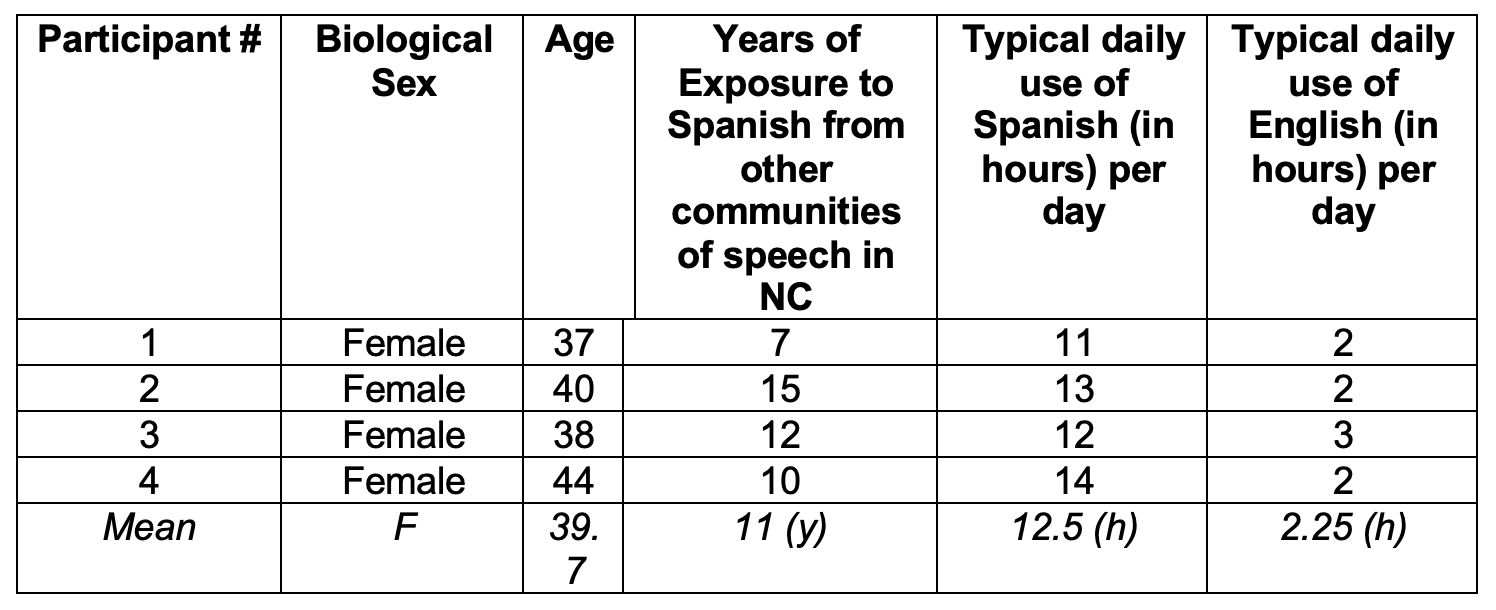
\includegraphics[width=6cm]{./includes/figures/background.png}
\caption{Background Information}\label{fig:vowels}
\end{center}
\end{figure}

\subsection{Acoustic Analysis}

Each participant generated 10 tokens and showed variability in the
articulation of syllable final liquids (refer to Figures 2 and 3 for
visual representations of waveforms and spectrograms, illustrating the
production of the /r/ in two participants across two target words).

\begin{figure}[!ht]
\begin{center}
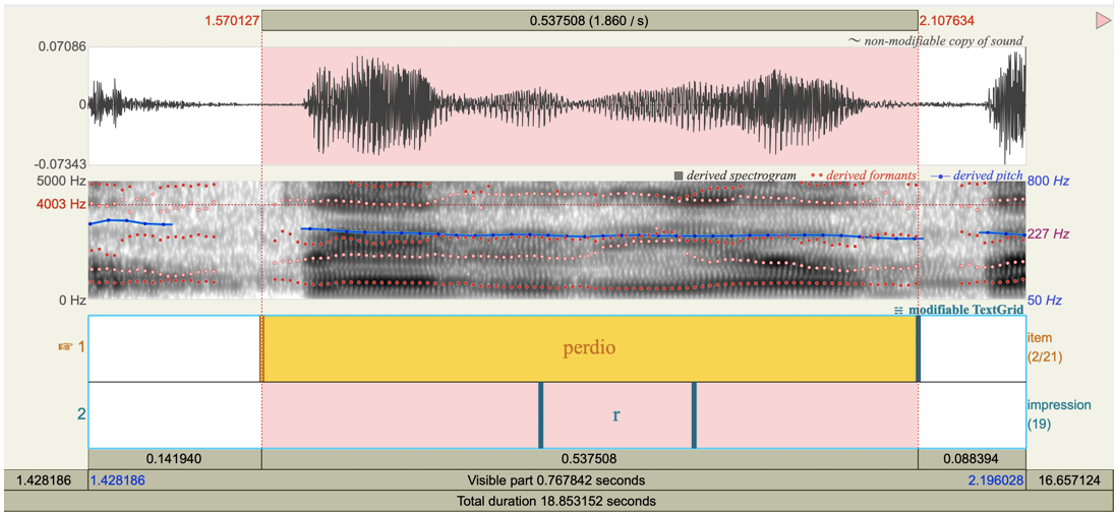
\includegraphics[width=6cm]{./includes/figures/praat.png}
\caption{Target word: “perdió” – participant 2}\label{fig:vowels}
\end{center}
\end{figure}

In Figure 2. the waveforms of participant 2, which can be identified on
the first row, show variability compared to those found in participant
3. Although the target words are not the same for both participants,
both could be lateralized. Participant 2, in this case, opted to produce
a tap sound /r/ , whereas participant 3 chose to lateralize the /r/ :
{[}pwélta{]}. Notably, the space allotted for /r/ production in
participant 2 shows two ``furry'' areas in the waveform, whereas in
participant 3, a ``flatter'' pattern is evident, resembling the
appearance of an /l/ sound. In regard to the spectrogram, which can be
observed in the second row in both speakers, participant 3 exhibited a
more fluctuant behavior in her F3 and F4 when lateralizing the /r/
sound, whereas in participant 2, it can be detected a more ``stable''
pattern in both formants. This may also suggest a method for identifying
lateralization processes through the use of spectrograms.

\begin{figure}[!ht]
\begin{center}
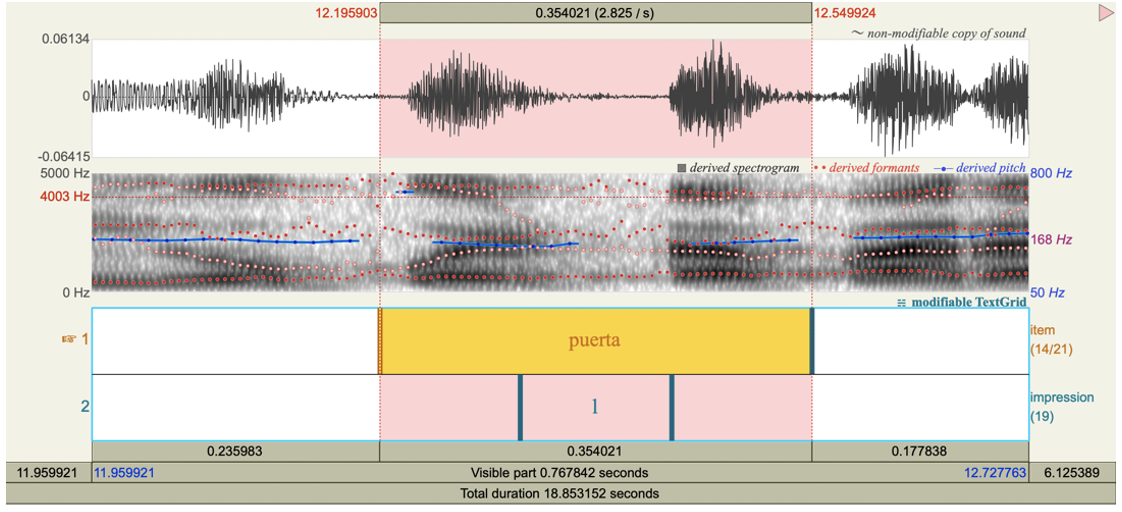
\includegraphics[width=6cm]{./includes/figures/praat1.png}
\caption{Target word: “puerta” – participant 3}\label{fig:vowels}
\end{center}
\end{figure}

During the four interviews, each participant showed different behaviors
while lateralizing the /r/ sound. Participant 1, for instance, did not
lateralize any of the /r/'s (she opted to produce taps in every token).
Participant 2, on the other hand, lateralized every /r/ sound in each
word. Participant 4 also lateralized most of the /r/ sounds, whereas
participant 3 showed almost equal production of taps and syllable final
liquids. See Figure 4. for a better understanding of the lateralization
processes and production of taps in every participant.

\begin{figure}[!ht]
\begin{center}
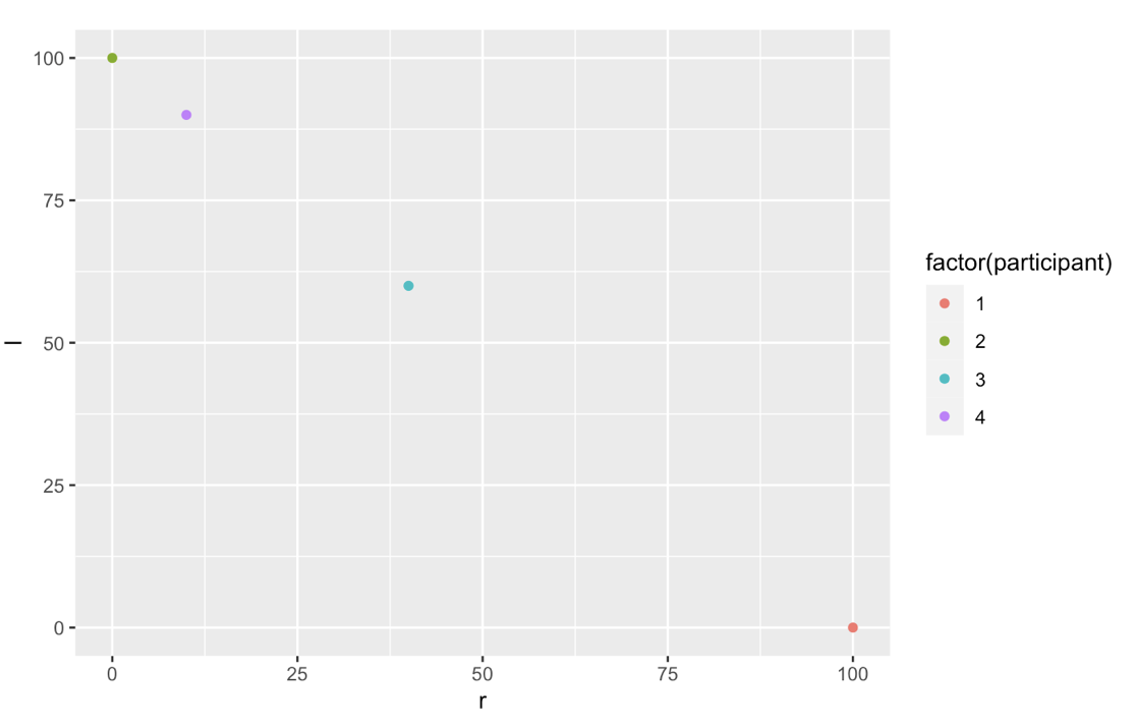
\includegraphics[width=6cm]{./includes/figures/graph.png}
\caption{Production of taps /r/ and /l/ in percentages per participant}\label{fig:vowels}
\end{center}
\end{figure}

The average values of formant trajectories were also examined to observe
the production of F3 and F4 in each participant. Figure 5 illustrates
the production of F3 in each subject (in Hertz), while Figure 6 depicts
the analysis of F4 production.

\begin{figure}[!ht]
\begin{center}
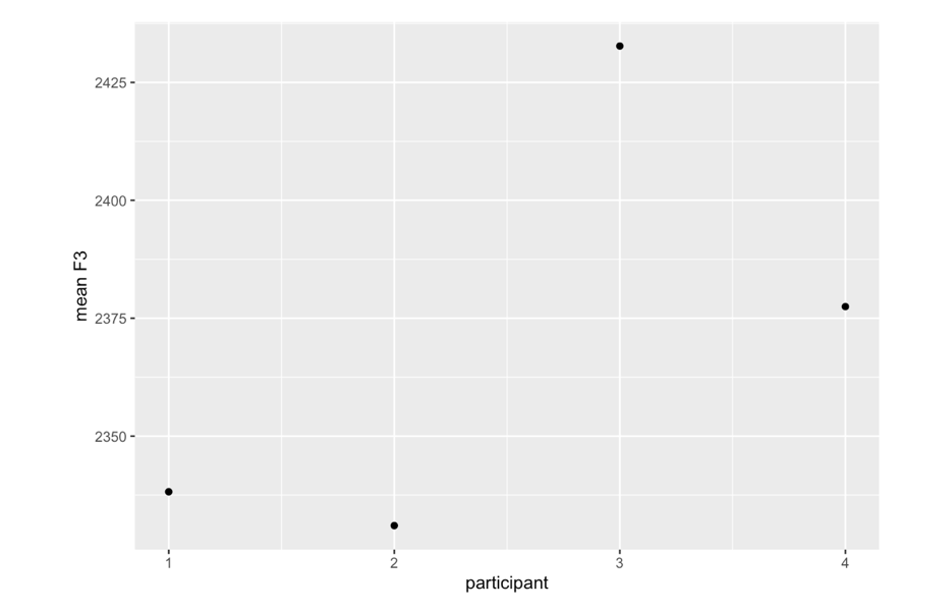
\includegraphics[width=6cm]{./includes/figures/graph1.png}
\caption{Mean of the concentration of acoustic energy in F3}\label{fig:vowels}
\end{center}
\end{figure}

\begin{figure}[!ht]
\begin{center}
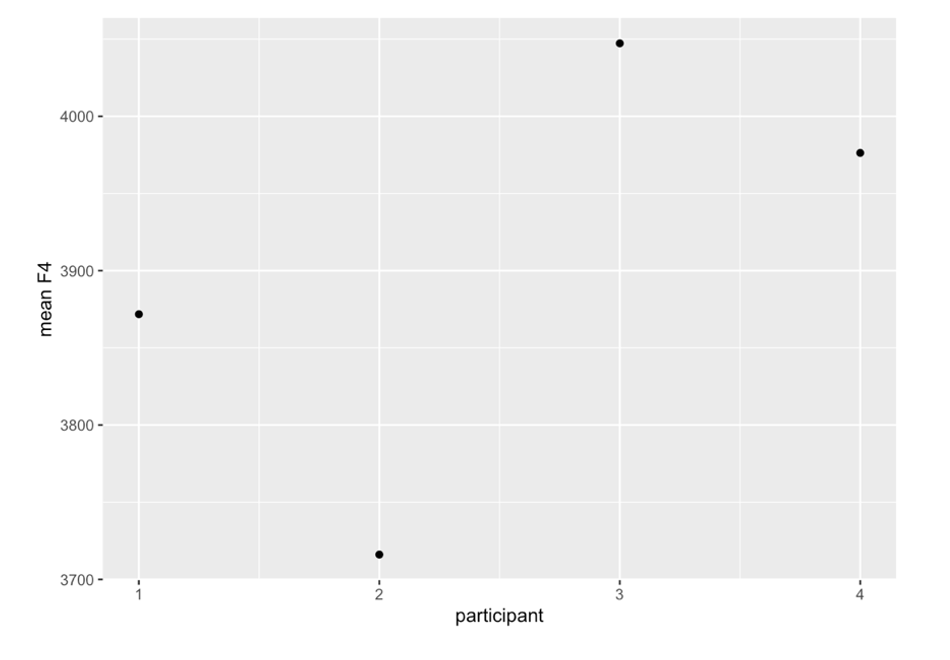
\includegraphics[width=6cm]{./includes/figures/graph2.png}
\caption{Mean of the concentration of acoustic energy in F4}\label{fig:vowels}
\end{center}
\end{figure}

Overall, participant 3 and 4 showed more concentration of acoustic
energy in formants 3 and 4. Participant 2, on her side, showed the
lowest production of acoustic energy in both formants. Participant 1
exhibited almost the lowest F3 and F4 out of the four speakers. See also
Figure 7. to observe the space plot (a graphical representation of data
points) of formants 3 and 4 in every participant considering the
production of individual tokens. In this last graph, it is relevant to
note that there is more consistency in some productions (participant 2
and 3), while others show more variation (participant 1).

\begin{figure}[!ht]
\begin{center}
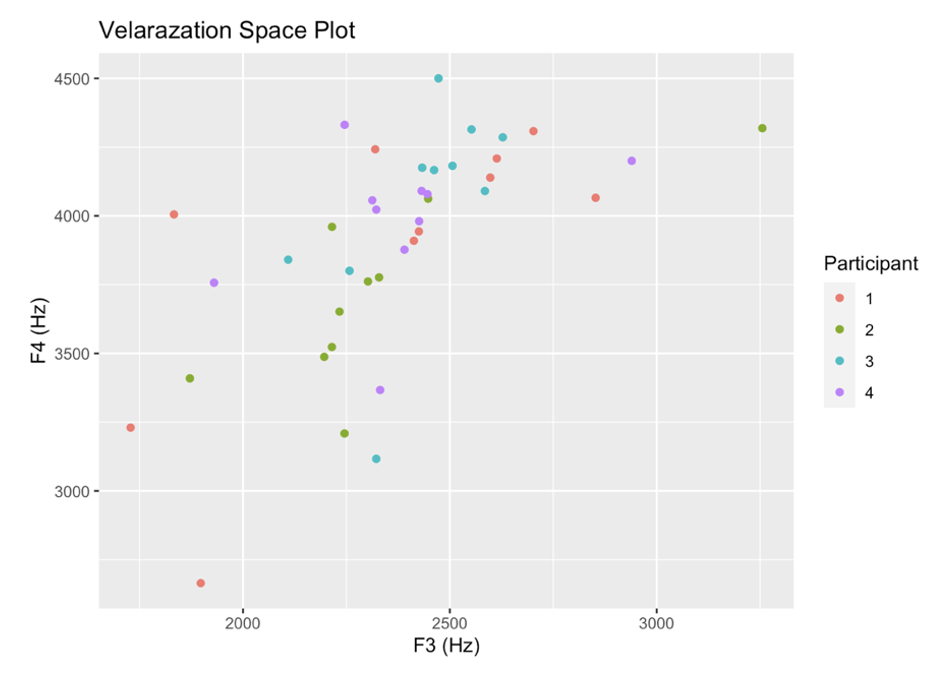
\includegraphics[width=6cm]{./includes/figures/graph3.png}
\caption{Mean of the concentration of acoustic energy in F3 and F4}\label{fig:vowels}
\end{center}
\end{figure}

\section{Discussion}

The results of this pilot study, surrounding four Puerto Rican women
living in North Carolina, reveal intriguing patterns in their
sociophonological behavior, negotiation of identity, and responses to
social dynamics when immersed in a multilingual context. Considering the
acoustic analysis, each participant showcased variety in the
articulation of syllable final liquids. Figures 1. and 2. explain these
variations through waveforms and spectrograms, highlighting differences
in articulation strategies across participants and target words.
Participant 1, for instance, steadily produced taps: /r/, while
participant 2 consistently lateralized /r/ sounds. Participant 4 showed
a similar trend to participant 2, whereas participant 3 exhibited a more
balanced production of taps and syllable final liquids. It is important
to note that this variability depends on positive and/or negative
experiences within their contexts. During the interview, participant 1
mentioned that when she reads sentences out loud, her teaching role
would come out, and that there was no room for lateralization.
Participant 4, on the other hand, did not show any lateralization during
the first couple of words, but then felt a little bit more ``confident''
(she mentioned it after having read the target words) and started
transforming the /r/ sounds into /l/ sounds. These results match with
the hypotheses stated earlier in the document. Alongside with the
previous ideas, analyzing formant trajectories revealed remarkable
insights into acoustic energy concentration. While participants 3 and 4
exhibited higher concentrations in formants 3 and 4, participant 2
displayed the lowest energy production in both formants (see Graph 4.).
This mechanism of comparing F3 and F4 through Praat, if expanded and/or
studied with more participants, may suggest a method for identifying
lateralization processes through the use of spectrograms.

\section{References}

\begin{itemize}
\item
  Alba, Orlando. (2016). Una Mirada Panorámica al Español Antillano.
  Books. 10. \url{https://scholarsarchive.byu.edu/books/10}
\item
  Carroll, K.S., Rivera, R.L., Santiago, K. (2015). Questioning
  Linguistic Imperialism: Language Use and Needs in a Puerto Rican
  Agriculture Program. In: Fabricius, A.H., Preisler, B. (eds)
  Transcultural Interaction and Linguistic Diversity in Higher
  Education. Palgrave Macmillan, London.
  \url{https://doi.org/10.1057/9781137397478_8}
\item
  Domínguez Rosado, B. (2015). The Unlinking of Language and Puerto
  Rican Identity: New Trends in Sight. Newcastle upon Tyne: Cambridge
  Scholars.Eckert, P. (2019). The limits of meaning: Social
  indexicality, variation, and the cline of interiority. Language 95(4),
  751-776.https://doi.org/10.1353/lan.2019.0072.
\item
  González-Rivera, M. \& L. A. Ortiz López. (2018). El español y el
  inglés en Puerto Rico: una polémica de más de un siglo. Centro
  Journal, 30(1), 106-131.
\item
  Hespos SJ, Piccin TB. To generalize or not to generalize: spatial
  categories are influenced by physical attributes and language. Dev
  Sci. 2009 Jan;12(1):88-95. doi: 10.1111/j.1467-7687.2008.00749.x.
  PMID: 19120416.
\item
  Kaushanskaya M, Blumenfeld HK, Marian V. The Language Experience and
  Proficiency Questionnaire (LEAP-Q): Ten years later. Biling (Camb
  Engl). 2020 Nov;23(5):945-950. doi: 10.1017/s1366728919000038. Epub
  2019 Apr 15. PMID: 33628083; PMCID: PMC7899192.
\item
  López Morales, H. (2004) ``Situación actual del español en Puerto
  Rico''. En: El español en el mundo. Anuario del Instituto Cervantes,
  253-276.
\item
  López Morales, H. (1983). Estratificación social del español de San
  Juan de Puerto Rico {[}Portada no disponible{]}. México: Universidad
  Nacional Autónoma, Instituto de Investigaciones Filológicas. ISBN:
  968-837-136-X.
\item
  Malavet, P. A. (2000). Puerto Rico: Cultural Nation, American Colony.
  Mich. J. Race \& L., 6, 1.
\item
  Oliver Rajan, J. (2022). El español de la zona cafetalera de Puerto
  Rico y sus narrativas orales como expresión identitaria. Borealis --
  An International Journal of Hispanic Linguistics, 11(2), 95--111.
  \url{https://doi.org/10.7557/1.11.2.6435}
\item
  Ortiz López, L. A. (2022). El español en Puerto Rico. In Dialectología
  hispánica / The Routledge Handbook of Spanish Dialectology (1st ed.,
  pp.~15). Routledge. \url{https://doi.org/10.4324/9780429294259}
\item
  Schmidt, J. R. (2014). The Politics of English in Puerto Rico's
  Schools. {[}Copyright © 2014{]}. ISBN: 978-1-935049-94-4
\item
  Schneider, A. M. (2013). Breves consideraciones sobre el sistema
  colonial en Puerto Rico. Revista História: Debates e Tendências,
  13(1), páginas 91-99.
\item
  Wardhaugh, R., \& Fuller, J. M. (2021). An Introduction to
  Sociolinguistics. (8 ed.) Wiley.
\end{itemize}

\bibliographystyle{./includes/bib/IEEEtran.bst}
\bibliography{./includes/bib/icphs2023.bib}

\theendnotes

\end{document}
